\documentclass{G7-32}

% --- Packages not provided by G7-32 ---

% Extra math symbols (amsmath is already loaded by G7-32)
\usepackage{amsfonts}
\usepackage{amssymb}

% Tables
\usepackage{booktabs}
\usepackage{array}

% Colors and extra TikZ libs (tikz is already loaded by G7-32)
\usepackage{xcolor}
\usetikzlibrary{arrows.meta, shapes.geometric, calc, fit, backgrounds}

% Source code listings
\usepackage{listings}
\lstset{
  basicstyle=\small\ttfamily,
  breaklines=true,
  frame=single,
  numbers=left,
  numberstyle=\tiny,
  showstringspaces=false,
  tabsize=4,
}

% Hyperlinks (load last, after all other packages)
\usepackage[colorlinks=true, linkcolor=black, citecolor=black, urlcolor=blue]{hyperref}

% -----------------------------------------------

\begin{document}

\setcounter{page}{3}
\tableofcontents
\clearpage

\chapter*{ВВЕДЕНИЕ}
\addcontentsline{toc}{chapter}{ВВЕДЕНИЕ}

\textbf{Актуальность темы.}
Робототехника является одной из наиболее динамично развивающихся областей современной техники.
Проектирование, верификация и тестирование робототехнических систем требуют значительных временных и финансовых затрат при работе с физическим оборудованием.
Программные симуляторы позволяют перенести большую часть этих работ в виртуальную среду, существенно сокращая цикл разработки и снижая риски.

Физическое моделирование — ключевой компонент любой симуляционной платформы.
Его задача состоит в воспроизведении динамики твёрдых тел, контактных взаимодействий и кинематических ограничений с точностью, достаточной для верификации алгоритмов управления.
Требования к производительности при этом постоянно растут: задачи обучения с подкреплением предполагают запуск тысяч параллельных симуляций, а построение цифровых двойников требует работы в режиме реального времени.
Графические процессоры (GPU), обладающие тысячами вычислительных ядер, открывают принципиально новые возможности для ускорения расчётов физической динамики.

В условиях ограничений на использование зарубежных программных продуктов актуальность создания отечественных инструментов робототехнической симуляции существенно возрастает.
Разработка программного комплекса «Модейлер» направлена на создание полноценной платформы для моделирования и тестирования робототехнических систем, ориентированной на задачи импортонезависимой инженерной разработки.
Физический движок с GPU-ускорением является одной из центральных подсистем этого комплекса.

\textbf{Степень научной разработанности.}
Задача физического моделирования твёрдых тел в робототехнике изучается начиная с 1990-х годов.
Основополагающие работы Д.~Барафа и А.~Уиткина~\cite{baraff1997physically} заложили теоретическую базу для моделирования контактной динамики.
На сегодняшний день существует ряд широко используемых библиотек физического моделирования: Bullet Physics~\cite{coumans2015bullet}, NVIDIA PhysX~\cite{physx2023}, MuJoCo~\cite{todorov2012mujoco}, ODE~\cite{smith2005ode} и Rapier~\cite{crozet2021rapier}.
В 2024 году компания NVIDIA анонсировала физический движок Newton~\cite{nvidia2024newton}, ориентированный на GPU-ускоренную симуляцию для задач робототехники.

Тем не менее перечисленные решения, как правило, не объединяют в одном продукте удобную среду визуального моделирования, высокоточную физическую симуляцию с масштабным GPU-ускорением и глубокую интеграцию с инструментами разработки робототехнических систем.
Кроме того, большинство из них распространяются на условиях лицензий, ограничивающих коммерческое или государственное применение.

\textbf{Цель исследования} — разработка подсистемы физического моделирования с поддержкой GPU-ускорения для применения в программном комплексе робототехнической симуляции «Модейлер».

\textbf{Задачи исследования:}
\begin{enumerate}
  \item провести анализ задач физической симуляции в робототехнике и требований к физическим движкам;
  \item выполнить сравнительный обзор существующих систем физического моделирования;
  \item определить функциональные и нефункциональные требования к разрабатываемой подсистеме;
  \item обосновать выбор алгоритмов динамики твёрдых тел, обнаружения столкновений и решения ограничений;
  \item разработать архитектуру физического движка и модуля GPU-ускорения;
  \item реализовать ядро физического движка и GPU-вычислительный модуль на основе Vulkan Compute;
  \item провести верификацию физической корректности и оценить производительность разработанной подсистемы.
\end{enumerate}

\textbf{Объект исследования} — программный комплекс моделирования робототехнических систем «Модейлер».

\textbf{Предмет исследования} — алгоритмы и программные средства физического моделирования динамики твёрдых тел с применением вычислений на графических процессорах.

\textbf{Практическая значимость.}
Разработанная подсистема является компонентом программного комплекса «Модейлер» и может применяться для:
верификации алгоритмов управления роботами в режиме software-in-the-loop;
построения цифровых двойников промышленных и мобильных робототехнических установок;
обучения нейросетевых систем управления методами обучения с подкреплением.
Применение GPU-ускорения позволяет многократно увеличить число одновременно моделируемых систем по сравнению с CPU-реализацией.

\textbf{Структура работы.}
Диссертация состоит из введения, пяти глав, заключения, списка использованных источников и приложений.

В первой главе проведён анализ предметной области: рассмотрены задачи физической симуляции в робототехнике, выполнен обзор существующих решений и сформулированы требования к разрабатываемой системе.

Вторая глава посвящена теоретическим основам: изложены уравнения механики твёрдого тела, рассмотрены алгоритмы обнаружения столкновений, методы численного интегрирования и модели контактной динамики.

В третьей главе представлены архитектура программного комплекса «Модейлер» и детальное проектирование физического движка и GPU-вычислительного модуля.

Четвёртая глава описывает реализацию: ядро физического движка, GPU-ускорение на основе Vulkan Compute и программные интерфейсы.

Пятая глава содержит результаты тестирования и оценку производительности.

\chapter{АНАЛИЗ ПРЕДМЕТНОЙ ОБЛАСТИ}

\section{Задачи физической симуляции в робототехнике}

В отличие от систем симуляции общего назначения, которые применяются в компьютерной графики и индустрии 
видеоигр, и в которых единственным критереем качества моделирумых процессов является видимая "натуральность" 
поведения объектов сцены, физическая симуляция в контексте робототехники предъявляет специфические требования 
к точности, воспроизводимости и интеграции с системами управления.

\subsection{Проектирования роботов}

Традиционным применением симуляции является верификация кинематических и динамических характеристик робота ещё 
на этапе проектирования. Расчёт динамики твёрдых тел позволяет оценить нагрузки на звенья и соединения, 
проверить досягаемость рабочей зоны и обнаружить потенциальные столкновения. Такой подход сокращает число 
физических прототипов и уменьшает стоимость разработки~\cite{siciliano2016springer}.

\subsection{Виртуальных испытаниях}

Методология software-in-the-loop (SIL) предполагает замкнутый цикл: программный модуль управления получает 
данные от виртуальных сенсоров, вырабатывает управляющие воздействия и передаёт их виртуальным 
приводам~\cite{bruyninckx2001open}. Физический движок при этом играет роль виртуальной среды, в которой 
исполняется реальный код управляющей программы.

Ключевым требованием SIL-тестирования является \emph{детерминированность}: при заданных начальных условиях и 
одинаковой управляющей программе симуляция должна давать воспроизводимые результаты. Это необходимо для 
отладки и автоматического тестирования алгоритмов управления.

Дополнительное требование --- \emph{работа в реальном времени} или близко к нему. Если один шаг симуляции 
занимает больше времени, чем реальный временной интервал, который он моделирует, обратная связь по управлению 
нарушается. Для типичного шага интегрирования 1~мс это означает, что полный цикл обработки одного шага должен 
укладываться в 1~мс на выбранной вычислительной платформе.

\subsection{Обучение с подкреплением}

Обучение с подкреплением (reinforcement learning, RL) стало мощным инструментом для синтеза управляющих 
политик в задачах локомоции, манипуляции и навигации~\cite{openai2019dexterous}. Обучение роботизированных 
агентов требует колоссального числа взаимодействий со средой: современные алгоритмы потребляют от $10^7$ до 
$10^9$ симуляционных шагов~\cite{mnih2015human}. При частоте симуляции 100~Гц это соответствует от 28 часов до 
278 лет вычислительного времени на одном потоке центрального процессора.

Решением является параллельный запуск тысяч независимых симуляций. Именно здесь использование графических 
процессоров приобретает принципиальное значение: их массово-параллельная архитектура позволяет одновременно 
выполнять сотни и тысячи экземпляров физических расчётов. В работе~\cite{liang2018gpu} показано, что 
реализация физической симуляции с использованием графического ускорителя обеспечивает ускорение от 10 до 100 
раз по сравнению с центральным процессором при использовании пакетного режима.

\subsection{Цифровые двойники}

Цифровой двойник (digital twin) — это динамически обновляемая виртуальная модель физической системы, 
синхронизированная с реальным объектом по данным сенсоров~\cite{grieves2014digital}. В контексте промышленной 
робототехники цифровые двойники применяются для мониторинга состояния оборудования, предиктивного обслуживания 
и оптимизации технологических процессов.

Для цифровых двойников физический движок должен обеспечивать:
\begin{itemize}
  \item достаточную точность для соответствия реальному поведению системы;
  \item возможность работы быстрее реального времени для прогнозирования состояния системы;
  \item простую интеграцию с потоками сенсорных данных (ROS2, OPC-UA и аналогичными протоколами).
\end{itemize}

\begin{figure}[t]
\centering
\begin{tabular}{cc}
  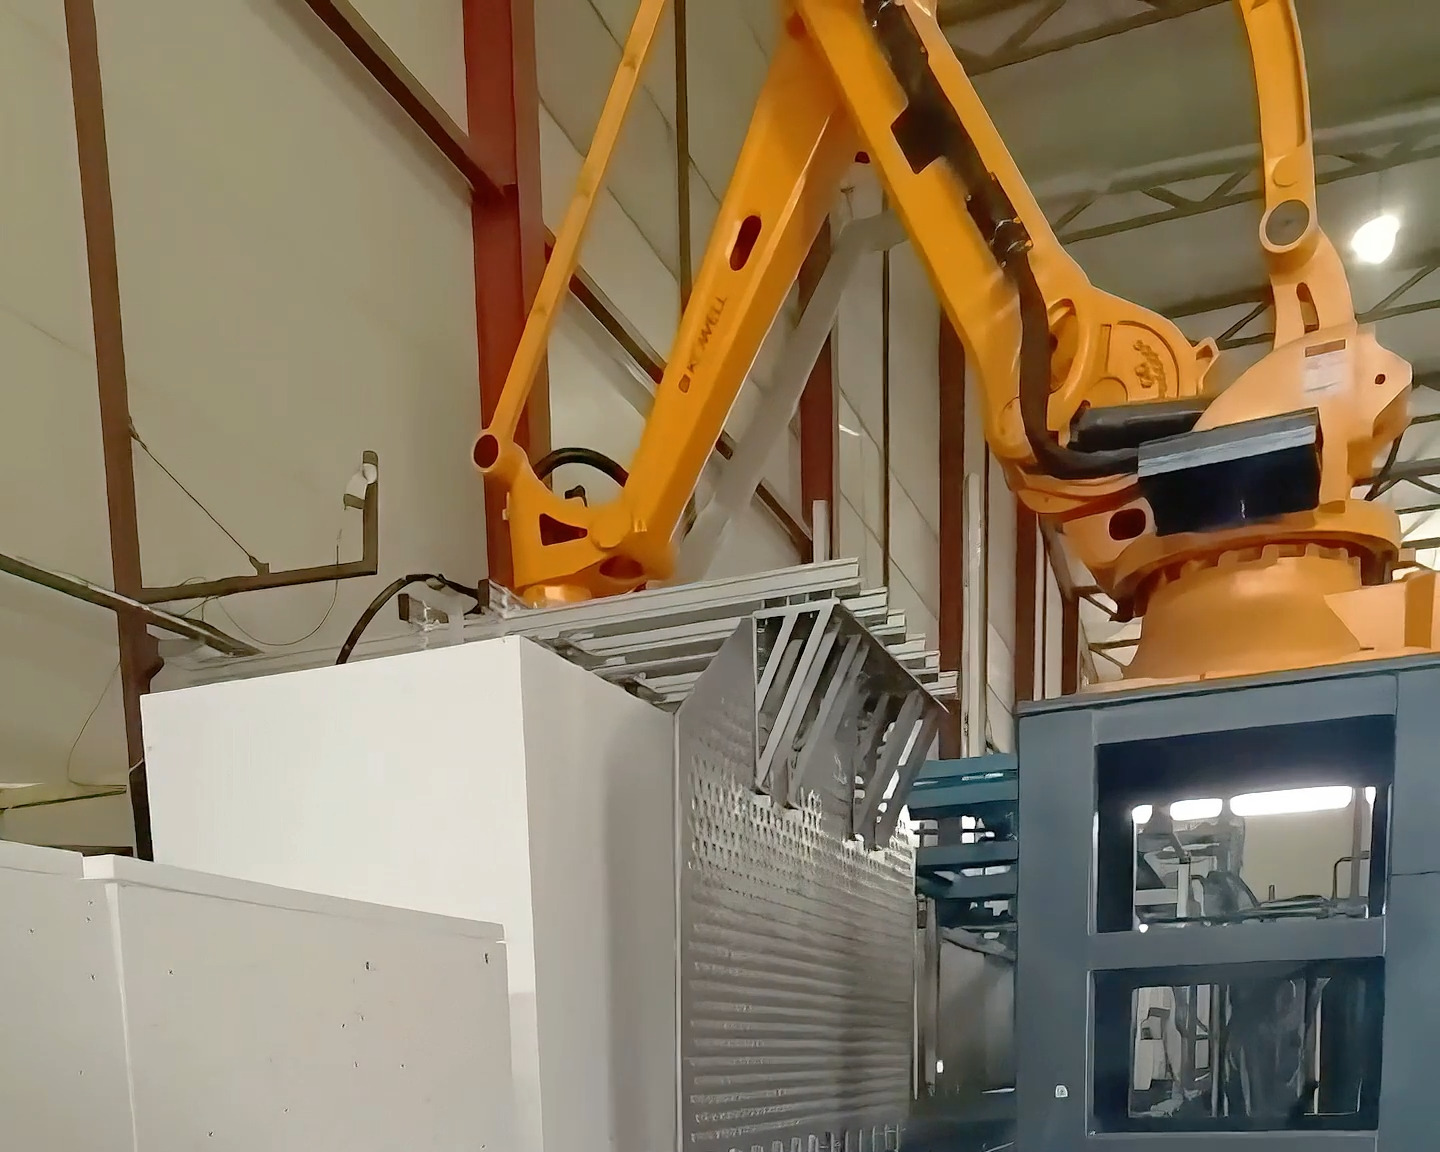
\includegraphics[width=0.44\textwidth]{figures/images/3DCloneEvroplast-real.jpg} &
  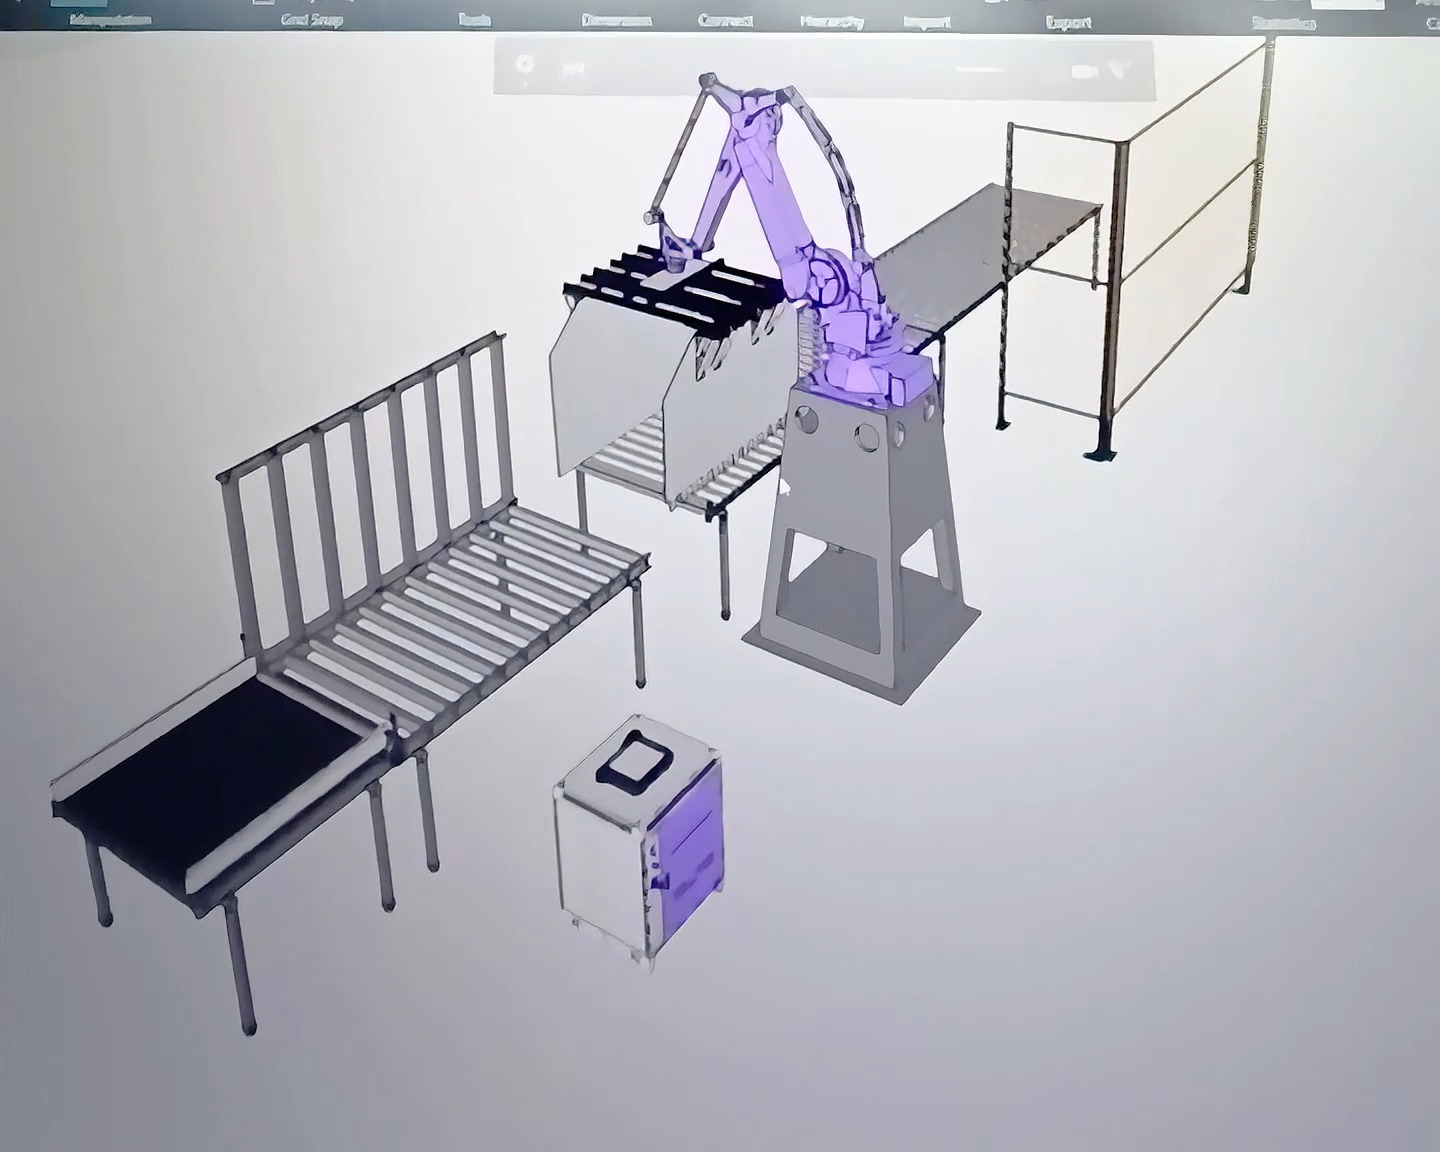
\includegraphics[width=0.44\textwidth]{figures/images/3DCloneEvroplast-double.jpg} \\
  а) реальный робот & б) цифровой двойник \\
\end{tabular}
\caption{Промышленный манипулятор и его цифровой двойник. Публикуется с разрешения ООО «Некстген Роботикс»}
\label{fig:digital_twin}
\end{figure}

\subsection{Выводы по разделу}

Таким образом, физическая симуляция в робототехнике решает качественно разные задачи --- от оффлайнового 
проектирования до обучения в реальном времени. Каждая задача предъявляет свои требования к физическому движку: 
SIL-тестирование требует детерминированности и работы в реальном времени, обучение с подкреплением --- 
максимальной производительности при запуске тысяч параллельных сред, цифровые двойники --- высокой точности и 
интеграции с внешними системами. Разрабатываемый физический движок должен удовлетворять всем перечисленным 
требованиям в рамках единой архитектуры.

\section{Обзор существующих систем физического моделирования}

На сегодняшний день существует ряд библиотек и систем физического моделирования, применяемых в 
робототехнических задачах. В данном разделе рассматриваются наиболее распространённые из них с акцентом на 
характеристики, релевантные для задач, сформулированных в разделе~1.1.

\subsection{Bullet Physics}

Bullet Physics~\cite{coumans2015bullet} --- библиотека с открытым исходным кодом, распространяемая под лицензией 
zlib. Она поддерживает симуляцию твёрдых тел, мягких тел и транспортных средств. Bullet использует импульсный 
решатель ограничений на основе алгоритма Projected Gauss-Seidel (PGS) и поддерживает несколько методов 
обнаружения столкновений.

Широкое использование Bullet в робототехнике обусловлено его интеграцией в симулятор 
Gazebo~\cite{koenig2004design} --- стандартный инструмент экосистемы ROS. Однако поддержка графического 
ускорителя в Bullet ограничена: исторически предлагалась экспериментальная реализация на CUDA для 
\textit{широкой фазы}, которая в дальнейшем не получила активного развития. Производительность "классической" 
реализации при числе тел свыше $10^3$ становится узким местом для задач обучения с подкреплением.

\subsection{NVIDIA PhysX}

NVIDIA PhysX~\cite{physx2023} --- коммерческая библиотека физического моделирования, исходный код которой 
доступен на GitHub под ограниченной лицензией. PhysX поддерживает аппаратное ускорение через CUDA, включая 
параллельную обработку тел и решение ограничений. Библиотека используется в симуляционных платформах Omniverse 
Isaac Sim, что делает её стандартом для задач робототехники с аппаратным ускорением на графическом процессоре.

Ограничения PhysX для разработки в рамках «Модейлера»: лицензия требует согласования для коммерческого и 
государственного применения; жёсткая привязка к стеку NVIDIA CUDA ограничивает поддержку оборудования; 
архитектура не рассчитана на замену отдельных компонентов собственными реализациями.

\subsection{MuJoCo}

MuJoCo (Multi-Joint dynamics with Contact)~\cite{todorov2012mujoco} --- физический движок, разработанный 
специально для задач робототехники и биомеханики. С 2021 года он доступен бесплатно; в 2022 году Google 
DeepMind открыла его исходный код.

Ключевые особенности MuJoCo:

\begin{itemize}
  \item использование обобщённых координат вместо декартовых повышает точность при моделировании кинематических цепей;
  \item собственный итерационный решатель ограничений, оптимизированный для сочленённых тел;
  \item поддержка симуляции сухого трения и деформируемых тел.
\end{itemize}

Поддержка графических ускорителей в MuJoCo реализована в виде экспериментального бэкенда MJX на основе 
JAX~\cite{mjx2023}, что ограничивает его применимость вне экосистемы Python/JAX.

\subsection{Open Dynamics Engine (ODE)}

ODE~\cite{smith2005ode} --- одна из первых библиотек физического моделирования с открытым исходным кодом, 
оказавшая значительное влияние на развитие отрасли. Она реализует решатель импульсов на основе 
LCP-формулировки (Linear Complementarity Problem) и поддерживает большое число видов сочленений.

На сегодняшний день ODE не получает активного развития: последний крупный релиз датируется 2017 годом. 
поддержка графических ускорителей отсутствует, производительность уступает современным решениям. Тем не менее 
ODE остаётся референсной реализацией для верификации результатов физического моделирования.

\subsection{Rapier}

Rapier~\cite{crozet2021rapier} --- современная библиотека физического моделирования, реализованная на языке 
Rust. Она обеспечивает высокую производительность и потокобезопасность благодаря модели владения памятью Rust. 
Rapier поддерживает параллельную обработку через SIMD-инструкции и многопоточность.

Поддержка вычислений на графических процессорах в Rapier в настоящее время не реализована. Библиотека 
ориентирована прежде всего на игровую индустрию и веб-разработку\footnote{Через трансляцию в WebAssembly}.

\subsection{NVIDIA Newton}

В 2024 году компания NVIDIA анонсировала физический движок Newton~\cite{nvidia2024newton}, разработанный 
совместно с Google DeepMind и Microsoft. Newton изначально ориентирован на использование графических 
ускорителей и задачи обучения роботов с подкреплением. Он построен на основе Warp (CUDA-ускоренный фреймворк 
на Python) и использует дифференцируемую физику для обучения.

На момент написания данной работы Newton находится на ранней стадии разработки и доступен с ограничениями. Его 
архитектура привязана к экосистеме Python/CUDA, графических ускорителям производства Nvidia и не предполагает 
использования в качестве встраиваемого компонента приложений на C++.

\subsection{Выводы по разделу}

Анализ существующих решений показывает, что ни одна из рассмотренных библиотек в полной мере не удовлетворяет 
совокупности требований проекта «Модейлер»:

\begin{itemize}
  \item свободная лицензия, допускающая коммерческое и государственное применение;
  \item полноценная поддержка вычислений на графических ускорителях разных производителей;
  \item C++ API для встраивания в мультиплатформенное настольное приложение;
  \item возможность расширения и адаптации под нужды конкретной платформы.
\end{itemize}

Это обосновывает разработку собственного физического движка \textit{dyphur}. В качестве ориентира при 
проектировании используются лучшие практики из рассмотренных систем:

\begin{itemize}
  \item позиционный метод решения ограничений (XPBD), зарекомендовавший себя в 
        симуляторах~\cite{macklin2016xpbd};
  \item параллельные BVH-алгоритмы из PhysX и Newton;
  \item открытая лицензия Apache~2.0 по образцу MuJoCo и Rapier, которая позволит сформировать вокруг проекта активное 
  сообщество.
\end{itemize}

\section{Анализ требований к разрабатываемой системе}

На основе анализа задач физической симуляции (раздел~1.1) и обзора существующих решений (раздел~1.2) сформулированы требования к физическому движку «Модейлера».
Требования разделены на функциональные (что система должна делать) и нефункциональные (как она должна это делать).

\subsection{Функциональные требования}

\paragraph{Моделирование твёрдых тел.}
Система должна поддерживать симуляцию произвольного числа твёрдых тел с заданными массово-инерционными характеристиками.
Каждое тело имеет шесть степеней свободы (три поступательные и три вращательные).
Поддерживается применение внешних сил и моментов.

\paragraph{Обнаружение столкновений.}
Система должна обнаруживать геометрические пересечения между телами и вычислять контактные точки, нормали и глубину проникновения.
Поддерживаемые примитивные геометрии: сфера, капсула, коробка (AABB/OBB), цилиндр, выпуклый многогранник.

\paragraph{Физика контактов и трения.}
Обработка контактов включает: нормальные импульсы (предотвращение взаимопроникновения) и касательные импульсы (кулоново трение).
Коэффициенты трения и упругости задаются на уровне пар материалов.

\paragraph{Кинематические связи (joints).}
Поддерживаются следующие типы сочленений: вращательное (revolute), призматическое (prismatic), фиксированное (fixed), шаровое (ball-and-socket).
Ограничения скорости, позиции и момента задаются на уровне сочленения.

\paragraph{Интеграция с ROS2.}
Движок должен предоставлять интерфейс для передачи данных о состоянии тел (поза, скорость, усилия) в систему ROS2 и приёма управляющих воздействий.

\paragraph{GPU-ускорение.}
Система должна поддерживать перенос вычислительно-ёмких этапов симуляции на GPU через API Vulkan Compute.
GPU-бэкенд должен быть опциональным: при его отсутствии система работает в CPU-режиме.

\paragraph{Параллельная симуляция.}
Движок должен поддерживать одновременную симуляцию нескольких независимых сцен (для задач обучения с подкреплением).
На GPU это реализуется через пакетную (batched) обработку сцен.

\subsection{Нефункциональные требования}

\paragraph{Производительность.}
Система должна обеспечивать симуляцию сцены с $N_b \leq 1000$ твёрдых тел в реальном времени ($\Delta t = 1\text{ мс}$) на типичной рабочей станции (8-ядерный CPU).
При использовании GPU время шага для пакета из 1000 независимых сцен с $N_b = 64$ телами должно быть не более 10~мс.

\paragraph{Детерминированность.}
При одинаковых начальных условиях и последовательности управляющих воздействий результаты симуляции должны быть воспроизводимы.
Для CPU-режима детерминированность гарантируется при фиксированном числе потоков; для GPU-режима — в пределах одного запуска на одном устройстве.

\paragraph{Точность.}
Физическая ошибка (отклонение от аналитического решения) для базовых тестовых сценариев (свободное падение, маятник, упругий удар) не должна превышать 1\% за 10 секунд симуляции при шаге интегрирования 1~мс.

\paragraph{Платформенная независимость.}
Движок реализуется на C++17 и должен компилироваться без модификаций под Linux x86-64 и Windows x86-64.
GPU-модуль использует Vulkan~1.3 как кроссплатформенный API, поддерживаемый на оборудовании AMD, NVIDIA и Intel.

\paragraph{Расширяемость.}
Архитектура должна допускать замену отдельных компонентов (солвера, алгоритма обнаружения столкновений) без изменения публичного API.
Это позволяет экспериментировать с альтернативными алгоритмами и адаптировать движок под конкретные задачи.

\paragraph{Интеграция в «Модейлер».}
Физический движок предоставляется как статически компонуемая библиотека (lib) с заголовочными файлами C++.
Зависимости ограничены стандартной библиотекой C++, математической библиотекой линейной алгебры и Vulkan SDK.

\subsection{Выводы по разделу}

Сформулированные требования охватывают все аспекты физического движка: базовую симуляционную функциональность, GPU-ускорение, точность и интеграцию с платформой.
Требования к производительности указывают на необходимость эффективной GPU-реализации и пакетной обработки сцен.
Требование кроссплатформенности и расширяемости определяет выбор Vulkan в качестве GPU API вместо CUDA, что отличает разрабатываемый движок от большинства аналогов.


\chapter{ТЕОРЕТИЧЕСКИЕ ОСНОВЫ}

\section{Механика твёрдого тела}

% TODO: Уравнения движения, тензор инерции, кватернионы для ориентации.

\section{Обнаружение столкновений}

% TODO: Иерархии AABB, алгоритмы GJK/EPA, вычисление контактных точек.

\section{Численное интегрирование уравнений движения}

% TODO: Symplectic Euler, Runge-Kutta, velocity Verlet; анализ устойчивости.

\section{Модель контактной динамики и решение ограничений}

% TODO: LCP-формулировка, импульсный метод, PGS-солвер, NNCG.

\chapter{АРХИТЕКТУРА И ПРОЕКТИРОВАНИЕ}

\section{Архитектура программного комплекса «Модейлер»}

\subsection{Общее описание платформы}

«Модейлер» — кроссплатформенная программная система для интерактивного моделирования и симуляции роботизированных устройств. Платформа предназначена для инженеров-разработчиков, исследователей и специалистов по автоматизации, решающих задачи верификации кинематических и динамических характеристик роботов без физического прототипирования.

В области промышленной робототехники задачи, для которых применяется «Модейлер», охватывают проектирование роботизированных ячеек, отладку управляющих алгоритмов в режиме программного замкнутого контура (SIL), а также подготовку траекторий движения. В сфере исследовательских и образовательных применений платформа обеспечивает возможность экспериментов с моделями на основе описания роботов в формате URDF\footnote{Unified Robot Description Format — стандартный XML-формат, используемый в экосистеме ROS.} без необходимости развёртывания реального оборудования.

В отличие от универсальных систем физического моделирования (рассмотренных в разделе~1.2), «Модейлер» ориентирован именно на робототехнические применения: нативная поддержка URDF-моделей, интеграция с ROS~2 и специализированный GPU-ускоренный физический движок составляют его ключевые характеристики.

\subsection{Многоуровневая архитектура}

Архитектура «Модейлера» организована по принципу строгого разделения ответственности, что отражается в выделении четырёх горизонтальных уровней: интерфейса пользователя, программного ядра, сцены и рендеринга, а также физического моделирования. Рисунок~\ref{fig:modeuler_architecture} иллюстрирует взаимодействие этих уровней.

\begin{figure}[h]
\centering
\begin{tikzpicture}[
  font=\small,
  layer/.style={
    draw, rounded corners=4pt,
    minimum width=11cm, minimum height=1.1cm,
    align=center, text width=10.5cm
  },
  grouplabel/.style={font=\footnotesize\itshape, text=gray},
  arr/.style={-{Stealth[length=6pt]}, thick},
]

% Layers (bottom to top)
\node[layer, fill=blue!10]   (gpu)     at (0,0)   {GPU-ускоренный физический движок\\{\footnotesize Vulkan Compute, SSBO, вычислительные шейдеры}};
\node[layer, fill=green!10]  (scene)   at (0,1.5) {Слой сцены и рендеринга\\{\footnotesize VulkanSceneGraph v1.1.14, vsgXchange, urdfdom}};
\node[layer, fill=yellow!10] (core)    at (0,3.0) {Программное ядро (C~ABI)\\{\footnotesize modeuler.h, управление сценой, Vulkan-устройство}};
\node[layer, fill=orange!10] (ui_win)  at (-2.75,4.5) {WPF / .NET~10\\{\footnotesize Windows}};
\node[layer, fill=orange!10, minimum width=5cm, text width=4.5cm] (ui_gtk)  at (2.75,4.5) {GTK~4 / C\\{\footnotesize Linux}};

% Arrows
\draw[arr] (gpu.north)   -- (scene.south);
\draw[arr] (scene.north) -- (core.south);
\draw[arr] (core.north) -- ++(0,0.55) -| (ui_win.south);
\draw[arr] (core.north) -- ++(0,0.55) -| (ui_gtk.south);

% Side labels
\node[grouplabel, right=0.3cm of gpu]   {§\,3.3};
\node[grouplabel, right=0.3cm of scene] {VSG};
\node[grouplabel, right=0.3cm of core]  {§\,3.1.3};

\end{tikzpicture}
\caption{Многоуровневая архитектура программного комплекса «Модейлер»}
\label{fig:modeuler_architecture}
\end{figure}

\textbf{Уровень пользовательского интерфейса.} Для обеспечения кроссплатформенности реализованы два независимых приложения верхнего уровня. Приложение для Windows построено на основе .NET~10 с использованием Windows Presentation Foundation (WPF) и библиотек Fluent.Ribbon и AvalonDock, обеспечивающих профессиональный пользовательский интерфейс с вкладками, плавающими панелями и лентой инструментов. Приложение для Linux реализовано на C с использованием GTK~4. Оба варианта взаимодействуют с ядром исключительно через C~ABI, что позволяет независимо развивать каждый из интерфейсов.

\textbf{Уровень программного ядра} предоставляет публичный стабильный интерфейс в виде заголовочного файла~\texttt{modeuler.h}, полностью совместимого со стандартом языка~C. Такое решение обеспечивает двоичную совместимость (ABI stability): интерфейсные типы используют только примитивные типы данных и непрозрачные указатели (\texttt{modeuler\_scene\_t}, \texttt{modeuler\_window\_t}), а все детали реализации на C++ скрыты за непрозрачным указателем. Внутри ядра располагается менеджер Vulkan-устройства — единственный экземпляр~\texttt{vsg::Instance} и связанное с ним~\texttt{vsg::Device}, создаваемые при первом обращении.

\textbf{Уровень сцены и рендеринга} реализован на основе VulkanSceneGraph~(VSG)~--- высокопроизводительной библиотеки визуализации, построенной непосредственно поверх Vulkan. VSG организует трёхмерную сцену в виде ориентированного ациклического графа (DAG), узлы которого соответствуют геометрическим преобразованиям, меш-данным и материалам. Для загрузки форматов 3D-геометрии используется плагин~vsgXchange; для парсинга описаний роботов --- библиотека~urdfdom, разработанная в рамках экосистемы ROS.

\textbf{Физический движок} --- новый компонент, разрабатываемый в рамках данной диссертационной работы. Он занимает нижний уровень архитектуры и взаимодействует со слоем сцены в обоих направлениях: получает от него структуру кинематической цепочки модели и передаёт обновлённые трансформации тел на каждом шаге симуляции.

\subsection{Кинематическая модель робота}

Описание робота в формате URDF задаёт дерево звеньев (\textit{links}) и сочленений (\textit{joints}). Каждое звено несёт информацию о визуальной геометрии, коллизионной геометрии и инерционных характеристиках; каждое сочленение определяет тип кинематической пары, её ось и пределы перемещения. Система поддерживает следующие типы сочленений:

\begin{itemize}
  \item \texttt{REVOLUTE} — вращательная пара с ограниченным углом;
  \item \texttt{CONTINUOUS} — вращательная пара без ограничения угла;
  \item \texttt{PRISMATIC} — поступательная пара;
  \item \texttt{FLOATING} — 6-DOF сочленение (свободное тело);
  \item \texttt{PLANAR} — движение в плоскости;
  \item \texttt{FIXED} — жёсткое соединение без степеней свободы.
\end{itemize}

После загрузки URDF-файла физический движок строит внутреннее представление кинематической цепочки: каждое звено становится объектом типа \texttt{RigidBody} (или статическим препятствием), а каждое сочленение --- ограничением (\textit{constraint}) в системе уравнений динамики.

\subsection{Программный интерфейс ядра}
\label{sec:core_api}

Программный интерфейс ядра спроектирован по принципу минимальной поверхности: пользовательский код работает только с непрозрачными дескрипторами и узким набором функций. Это позволяет изменять внутреннюю реализацию без нарушения обратной совместимости.

\begin{lstlisting}[language=C, caption={Ключевые функции публичного C-интерфейса «Модейлера»}]
/* Инициализация и завершение работы */
modeuler_result_t modeuler_init(void);
void              modeuler_deinit(void);

/* Управление сценой */
modeuler_scene_t  modeuler_scene_create(void);
void              modeuler_scene_destroy(modeuler_scene_t scene);

/* Загрузка модели и создание физических тел */
modeuler_model_t  modeuler_model_import(modeuler_scene_t scene,
                                        const char *urdf_path);

/* Управление окном отображения */
modeuler_window_t modeuler_window_attach_native(
                      modeuler_scene_t scene,
                      void *native_handle,
                      modeuler_native_type_t type);

/* Шаг симуляции */
modeuler_result_t modeuler_physics_step(modeuler_scene_t scene,
                                        double dt);

/* Рендеринг кадра */
modeuler_result_t modeuler_run_frame(modeuler_window_t window);
\end{lstlisting}

Функция \texttt{modeuler\_physics\_step} вызывается управляющим циклом приложения с фиксированным шагом~$\Delta t$ (типично 1--2\,мс для реального времени). Результаты шага симуляции (обновлённые трансформации тел) немедленно применяются к VSG-узлам, после чего вызов~\texttt{modeuler\_run\_frame} генерирует новый кадр изображения.

Привязки для управляемых языков формируются инструментом~ClangSharp, который разбирает заголовочный файл~\texttt{modeuler.h} и генерирует код P/Invoke на языке~C\# для интеграции с WPF-приложением.

\subsection{Взаимодействие с ROS~2}

Интеграция с ROS~2 реализуется на двух уровнях. На уровне форматов данных: «Модейлер» использует URDF~--- официальный формат описания роботов в экосистеме ROS, а система координат при загрузке трансформаций соответствует конвенции фреймов~TF2. На уровне обмена данными: физический движок публикует состояние сочленений (\textit{joint states}), одометрию и показания сенсоров через топики ROS~2, что позволяет использовать «Модейлер» в качестве имитатора для управляющего программного обеспечения, работающего в штатной среде ROS~2 без каких-либо изменений кода.

\section{Проектирование физического движка}

\subsection{Концептуальная модель физического мира}

Физический движок оперирует понятием \textit{физического мира} (\texttt{PhysicsWorld}) --- изолированного пространства симуляции, содержащего все объекты сцены. Мир является единственным владельцем всех создаваемых объектов: тел, коллайдеров и ограничений. Такая архитектура с единственной точкой владения (ownership) исключает висячие ссылки и упрощает сериализацию состояния для целей воспроизводимой симуляции.

Физический мир характеризуется следующими глобальными параметрами:
\begin{itemize}
  \item вектор гравитационного ускорения $\mathbf{g}$ (по умолчанию $(0, 0, -9{,}81)$\,м/с²);
  \item шаг интегрирования $\Delta t$ (фиксированный или переменный с ограничением сверху);
  \item число итераций решателя ограничений $n_{\text{iter}}$;
  \item флаг включения GPU-ускорения и число параллельных потоков.
\end{itemize}

\subsection{Представление твёрдых тел}
\label{sec:rigid_body}

Твёрдое тело (\texttt{RigidBody}) является центральным объектом физической симуляции. Его состояние полностью определяется набором атрибутов, перечисленных в таблице~\ref{tab:rigidbody_state}.

\begin{table}[h]
\centering
\caption{Атрибуты состояния объекта \texttt{RigidBody}}
\label{tab:rigidbody_state}
\begin{tabular}{lll}
\toprule
\textbf{Атрибут} & \textbf{Тип} & \textbf{Описание} \\
\midrule
\texttt{position}        & $\mathbb{R}^3$  & Положение центра масс в мировых координатах \\
\texttt{orientation}     & $\mathbb{H}^1$  & Единичный кватернион ориентации \\
\texttt{linear\_vel}     & $\mathbb{R}^3$  & Линейная скорость центра масс \\
\texttt{angular\_vel}    & $\mathbb{R}^3$  & Угловая скорость в мировых координатах \\
\texttt{inv\_mass}       & $\mathbb{R}$    & Обратная масса ($0$ для статических тел) \\
\texttt{inv\_inertia}    & $\mathbb{R}^{3\times3}$ & Обратный тензор инерции в локальных координатах \\
\texttt{force\_accum}    & $\mathbb{R}^3$  & Накопленная сила за текущий шаг \\
\texttt{torque\_accum}   & $\mathbb{R}^3$  & Накопленный момент за текущий шаг \\
\texttt{restitution}     & $[0,1]$         & Коэффициент упругости при ударе \\
\texttt{friction}        & $\mathbb{R}^+$  & Коэффициент трения Кулона \\
\texttt{is\_static}      & \texttt{bool}   & Признак статического (бесконечно массивного) тела \\
\texttt{is\_sleeping}    & \texttt{bool}   & Признак неактивного тела \\
\bottomrule
\end{tabular}
\end{table}

Обратная масса $m^{-1}$ используется вместо прямого хранения массы, так как это исключает деление в вычислениях горячего пути и позволяет естественно представить статические тела ($m^{-1} = 0$) без специальных проверок. Аналогично, для тензора инерции хранится обратная матрица в локальных координатах тела $\mathbf{I}_{\text{body}}^{-1}$; пересчёт в мировые координаты производится через матрицу вращения по формуле, рассмотренной в разделе~2.1.

\textit{Режим сна} (\textit{sleeping}) позволяет пропускать симуляцию тел, кинетическая энергия которых опустилась ниже заданного порога за несколько последовательных шагов. Тело переводится обратно в активное состояние при любом контакте с другим активным телом или при воздействии внешней силы. Данный механизм критически важен для производительности сцен с большим числом тел, большинство из которых в типичный момент времени находятся в покое.

\subsection{Коллайдеры и примитивы столкновений}
\label{sec:colliders}

Коллайдер (\texttt{Collider}) определяет геометрическую форму тела для целей обнаружения столкновений и, как правило, является упрощённым представлением визуальной геометрии. Движок поддерживает иерархию коллайдеров, показанную на рисунке~\ref{fig:collider_hierarchy}.

\begin{figure}[h]
\centering
\begin{tikzpicture}[
  font=\small,
  box/.style={draw, rounded corners=3pt, minimum width=3cm, minimum height=0.7cm,
              align=center, fill=white},
  basebox/.style={draw, rounded corners=3pt, minimum width=4cm, minimum height=0.7cm,
                  align=center, fill=gray!15},
  arr/.style={-{Stealth[length=5pt]}, thick},
]

\node[basebox] (base) at (0,0) {\texttt{Collider} (абстрактный)};

\node[box] (sphere)  at (-5.5,-1.7) {\texttt{SphereCollider}};
\node[box] (capsule) at (-2.5,-1.7) {\texttt{CapsuleCollider}};
\node[box] (box)     at (0.5,-1.7)  {\texttt{BoxCollider}};
\node[box] (cvx)     at (3.5,-1.7)  {\texttt{ConvexHullCollider}};
\node[box] (mesh)    at (6.5,-1.7)  {\texttt{TriMeshCollider}};

\draw[arr] (base.south) -- ++(-5.5,-0.6) -- (sphere.north);
\draw[arr] (base.south) -- ++(-2.5,-0.6) -- (capsule.north);
\draw[arr] (base.south) -- ++(0.5,-0.6)  -- (box.north);
\draw[arr] (base.south) -- ++(3.5,-0.6)  -- (cvx.north);
\draw[arr] (base.south) -- ++(6.5,-0.6)  -- (mesh.north);

\end{tikzpicture}
\caption{Иерархия типов коллайдеров физического движка}
\label{fig:collider_hierarchy}
\end{figure}

\textbf{SphereCollider} задаётся радиусом и смещением центра относительно центра масс тела. Это простейший примитив: алгоритм столкновения двух сфер сводится к сравнению расстояния между центрами с суммой радиусов.

\textbf{CapsuleCollider} --- цилиндр с полусферическими торцами, задаётся радиусом и длиной оси. Хорошо аппроксимирует звенья манипуляторов, конечности роботов и трубообразные конструкции при низкой стоимости проверки столкновений.

\textbf{BoxCollider} (ориентированный параллелепипед, OBB) задаётся тремя полуразмерами вдоль осей локальной системы координат тела. Эффективен для прямоугольных конструкций.

\textbf{ConvexHullCollider} представляет выпуклую оболочку набора точек. Алгоритм GJK, рассмотренный в разделе~2.2, работает с любым выпуклым телом через функцию опоры; выпуклая оболочка является наиболее точным приближением произвольной геометрии, для которого GJK гарантированно применим.

\textbf{TriMeshCollider} --- произвольная невыпуклая сетка треугольников. Используется только для статических тел (пол, стены, неподвижные препятствия), так как столкновение двух произвольных невыпуклых тел требует разбиения на выпуклые части. Проверка столкновения с динамическим телом производится перебором по треугольникам с ускорением через BVH (\textit{Bounding Volume Hierarchy}).

Каждый коллайдер хранит смещение (\texttt{offset}) и ориентацию (\texttt{offset\_rotation}) относительно центра масс тела, что позволяет прикреплять несколько коллайдеров к одному телу и точнее аппроксимировать сложную геометрию.

\subsection{Ограничения и сочленения}
\label{sec:constraints}

Ограничения (\textit{constraints}) реализуют связи между парами тел. В рамках данного раздела рассмотрена классификация и структура данных; математическая формулировка дана в разделе~2.4.

Базовый класс \texttt{Constraint} задаёт интерфейс, используемый решателем:

\begin{lstlisting}[language=C++, caption={Интерфейс базового класса ограничения}]
class Constraint {
public:
    RigidBody *bodyA, *bodyB;  // nullptr для мирового фрейма

    // Вычислить якобиан J и вектор смещения b для данного шага
    virtual void computeJacobian(JacobianBlock &J, float b[],
                                 float dt) const = 0;

    // Нижняя и верхняя границы импульса (для трения и упоров)
    virtual void impulseLimits(float lo[], float hi[],
                               const float lambda[]) const = 0;
};
\end{lstlisting}

Конкретные классы ограничений, реализуемые в движке:

\begin{itemize}
  \item \texttt{ContactConstraint} --- создаётся автоматически при обнаружении столкновения: одно нормальное и до двух тангенциальных (фрикционных) ограничений;
  \item \texttt{RevoluteJoint} --- вращательная пара: фиксирует 5 из 6 степеней свободы, оставляя одну ось вращения; поддерживает пределы угла и мотор с заданной скоростью/моментом;
  \item \texttt{PrismaticJoint} --- поступательная пара вдоль одной оси;
  \item \texttt{FixedJoint} --- жёсткое соединение (6 ограничений), применяется для объединения нескольких тел в составное;
  \item \texttt{BallJoint} --- шаровое сочленение (фиксирует 3 трансляционные степени свободы);
  \item \texttt{DistanceConstraint} --- поддерживает фиксированное или ограниченное расстояние между двумя точками тел.
\end{itemize}

\subsection{Жизненный цикл шага симуляции}
\label{sec:sim_step}

Каждый шаг симуляции длительностью $\Delta t$ выполняется в строго определённой последовательности, схематически представленной на рисунке~\ref{fig:sim_pipeline}.

\begin{figure}[h]
\centering
\begin{tikzpicture}[
  font=\small,
  simstep/.style={draw, rounded corners=3pt, fill=white,
               minimum width=8cm, minimum height=0.75cm, align=center},
  gpustep/.style={draw, rounded corners=3pt, fill=blue!10,
              minimum width=8cm, minimum height=0.75cm, align=center},
  arr/.style={-{Stealth[length=6pt]}, thick},
  note/.style={font=\footnotesize\itshape, text=gray, align=left},
]

\node[simstep] (forces)   at (0,0)    {1. Применение внешних сил и гравитации};
\node[gpustep] (broad)    at (0,-1.1) {2. Широкая фаза обнаружения столкновений (GPU)};
\node[gpustep] (narrow)   at (0,-2.2) {3. Узкая фаза: GJK/EPA (GPU, параллельно по парам)};
\node[simstep] (warmstart)at (0,-3.3) {4. Warm-starting: перенос импульсов с прошлого шага};
\node[gpustep] (solver)   at (0,-4.4) {5. Итерационный решатель PGS (GPU)};
\node[simstep] (integrate)at (0,-5.5) {6. Симплектическое интегрирование положений};
\node[simstep] (sleep)    at (0,-6.6) {7. Обновление режима сна тел};
\node[simstep] (sync)     at (0,-7.7) {8. Передача трансформаций в слой сцены};

\foreach \a/\b in {forces/broad, broad/narrow, narrow/warmstart,
                    warmstart/solver, solver/integrate,
                    integrate/sleep, sleep/sync}
  \draw[arr] (\a.south) -- (\b.north);

\node[note, right=0.5cm of broad]    {§\,3.3};
\node[note, right=0.5cm of narrow]   {§\,3.3};
\node[note, right=0.5cm of solver]   {§\,3.3};

\end{tikzpicture}
\caption{Последовательность вычислений в рамках одного шага симуляции (голубым выделены стадии с GPU-ускорением)}
\label{fig:sim_pipeline}
\end{figure}

\textbf{Стадия 1.} Для каждого активного тела интегратор вычисляет предварительную скорость $\mathbf{v}^* = \mathbf{v} + m^{-1}\mathbf{F}_{\text{ext}}\Delta t$, где $\mathbf{F}_{\text{ext}}$ включает гравитацию и любые силы, приложенные пользовательским кодом. Эта предварительная скорость используется в качестве начального приближения для решателя.

\textbf{Стадии 2--3.} Обнаружение столкновений выполняется на GPU в два этапа (подробно рассмотрено в разделах~2.2 и~3.3). На выходе формируется список \textit{контактных точек} --- структур, содержащих нормаль, глубину проникновения, опорные точки на каждом теле и идентификаторы пары тел.

\textbf{Стадия 4.} Warm-starting (тёплый запуск) использует импульсы $\lambda$ из предыдущего шага в качестве начального приближения для итерационного решателя. Для каждого контакта, идентифицированного по хэшу пары (bodyA, bodyB, featureId), накопленный импульс немедленно применяется к скоростям тел, сокращая необходимое число итераций решателя.

\textbf{Стадия 5.} Решатель PGS (рассмотренный в разделе~2.4) выполняет $n_{\text{iter}}$ итераций; на GPU каждая итерация обрабатывает все независимые ограничения параллельно (подробнее в разделе~3.3).

\textbf{Стадия 6.} Симплектическое интегрирование Эйлера обновляет положения и ориентации:
\begin{align}
  \mathbf{r}(t + \Delta t) &= \mathbf{r}(t) + \mathbf{v}(t + \Delta t)\,\Delta t, \\
  \mathbf{q}(t + \Delta t) &= \text{norm}\!\left(\mathbf{q}(t) + \tfrac{1}{2}\boldsymbol{\Omega}(\boldsymbol{\omega}(t+\Delta t))\,\mathbf{q}(t)\,\Delta t\right).
\end{align}

\textbf{Стадия 7.} Энергетическое пороговое значение $E_{\text{sleep}} = \frac{1}{2}(m|\mathbf{v}|^2 + \boldsymbol{\omega}^T\mathbf{I}\boldsymbol{\omega})$ сравнивается с порогом; при превышении счётчик неактивности сбрасывается.

\textbf{Стадия 8.} Матрицы преобразования всех тел записываются в VSG-узлы сцены. Эта операция выполняется на CPU и является единственной точкой синхронизации между физическим движком и подсистемой рендеринга.

\subsection{Хранение данных в памяти}

Для эффективного GPU-вычисления тела и их атрибуты хранятся в структурах, ориентированных на массивный параллелизм. Вместо объектно-ориентированного представления «одна структура --- одно тело» используется шаблон \textit{Structure of Arrays} (SoA): каждый атрибут всех тел хранится в отдельном непрерывном массиве.

\begin{lstlisting}[language=C++, caption={Структура хранения данных тел (SoA-формат)}]
struct RigidBodyData {
    // Кинематические данные
    std::vector<glm::vec3>  positions;       // [N]
    std::vector<glm::quat>  orientations;    // [N]
    std::vector<glm::vec3>  linear_vels;     // [N]
    std::vector<glm::vec3>  angular_vels;    // [N]

    // Инерционные данные (загружаются один раз)
    std::vector<float>      inv_masses;      // [N]
    std::vector<glm::mat3>  inv_inertias;    // [N]

    // Приложенные силы (сбрасываются каждый шаг)
    std::vector<glm::vec3>  force_accums;    // [N]
    std::vector<glm::vec3>  torque_accums;   // [N]

    // Флаги состояния (упакованы побитово)
    std::vector<uint32_t>   flags;           // [N/32]
};
\end{lstlisting}

SoA-формат обеспечивает последовательный доступ к памяти при обработке массива тел, что критично как для CPU-кэша, так и для GPU-вейвфронтов. При передаче данных в GPU все массивы копируются в единый~SSBO (Shader Storage Buffer Object), разметка которого подробно рассмотрена в разделе~3.3.

\section{Проектирование GPU-вычислительного модуля}

\subsection{Обоснование выбора Vulkan Compute}

Для реализации GPU-ускорения физического движка были рассмотрены четыре основных технологии: CUDA, OpenCL, Metal Compute и Vulkan Compute. Выбор технологии определяется требованиями к кроссплатформенности, интеграции с существующим рендерингом и возможности использования единого GPU-устройства для симуляции и визуализации.

CUDA обеспечивает наилучшую производительность и богатейшую экосистему инструментов (Thrust, cuBLAS, cuSPARSE), однако ограничена исключительно оборудованием NVIDIA, что нарушает требование кроссплатформенности~--- один из ключевых принципов архитектуры «Модейлера».

OpenCL является открытым стандартом с поддержкой широкого класса ускорителей, однако его развитие фактически заморожено: последняя значимая версия спецификации (OpenCL~3.0) вышла в 2020~г., и крупнейшие поставщики GPU de facto перенесли акцент на проприетарные или Vulkan-основанные решения~\cite{vulkan13spec}.

Metal~Compute доступен только на платформах Apple и поэтому не рассматривается.

\textbf{Vulkan Compute} выбран как основная технология GPU-ускорения. Его преимущества в контексте данной работы:
\begin{enumerate}
  \item \textit{Интеграция с рендерингом.} VulkanSceneGraph уже инициализирует Vulkan-устройство; вычислительные конвейеры разделяют с рендерингом логическое устройство (\texttt{vk::Device}), очереди и буферную память, исключая копирование через системную шину.
  \item \textit{Кроссплатформенность.} Vulkan поддерживается на Windows (NVIDIA, AMD, Intel), Linux и Android.
  \item \textit{Явное управление синхронизацией.} Примитивы Vulkan (fence, semaphore, pipeline barrier) позволяют точно задать порядок исполнения между вычислительными и графическими командами.
  \item \textit{Шейдеры в формате SPIR-V.} Единое промежуточное представление позволяет компилировать шейдеры из GLSL при сборке и распространять бинарные SPIR-V модули.
\end{enumerate}

\subsection{Организация вычислительного конвейера}

GPU-модуль состоит из трёх независимых вычислительных конвейеров (\textit{compute pipelines}), соответствующих трём стадиям симуляционного шага, выполняемым на GPU (рис.~\ref{fig:sim_pipeline}): широкой фазе, узкой фазе и решателю. Каждый конвейер включает один или несколько вычислительных шейдеров (GLSL compute shaders, скомпилированных в SPIR-V).

Рисунок~\ref{fig:gpu_pipeline} показывает граф вычислений для одного шага симуляции.

\begin{figure}[h]
\centering
\begin{tikzpicture}[
  font=\small,
  cpubox/.style={draw, rounded corners=3pt, fill=orange!15,
                 minimum width=5.5cm, minimum height=0.75cm, align=center},
  gpubox/.style={draw, rounded corners=3pt, fill=blue!15,
                 minimum width=5.5cm, minimum height=0.75cm, align=center},
  barrierbox/.style={draw, dashed, fill=gray!10,
                     minimum width=5.5cm, minimum height=0.5cm, align=center,
                     font=\footnotesize\itshape},
  arr/.style={-{Stealth[length=5pt]}, thick},
  label/.style={font=\footnotesize, text=gray},
]

% CPU side
\node[cpubox] (cpu_prep)   at (-3.2, 0)    {CPU: обновление SSBO (SoA данные)};
\node[cpubox] (cpu_sync)   at (-3.2,-6.6)  {CPU: чтение результатов SSBO};
\node[cpubox] (cpu_scene)  at (-3.2,-7.7)  {CPU: обновление трансформаций VSG};

% GPU side
\node[gpubox] (broad)      at (3.2,-1.1)   {Broadphase: AABB-пары};
\node[barrierbox] (bar1)   at (3.2,-2.0)   {pipeline barrier};
\node[gpubox] (narrow)     at (3.2,-3.1)   {Narrowphase: GJK/EPA};
\node[barrierbox] (bar2)   at (3.2,-4.0)   {pipeline barrier};
\node[gpubox] (solver)     at (3.2,-5.1)   {PGS-solver ($n$ итераций)};
\node[barrierbox] (bar3)   at (3.2,-6.0)   {pipeline barrier};

% Arrows CPU->GPU and back
\draw[arr] (cpu_prep.east)  -- ++(0.5,0) |- (broad.west)
    node[midway, above, label] {vkCmdCopyBuffer};
\draw[arr] (solver.south) -- ++(0,-0.2) -| (-3.2,-6.35)
    node[midway, below, label] {fence};
\draw[arr] (cpu_sync.south) -- (cpu_scene.north);

% Arrows within GPU
\draw[arr] (broad.south) -- (bar1.north);
\draw[arr] (bar1.south)  -- (narrow.north);
\draw[arr] (narrow.south)-- (bar2.north);
\draw[arr] (bar2.south)  -- (solver.north);
\draw[arr] (solver.south)-- (bar3.north);

% Labels
\node[label, left=0.3cm of cpu_prep]  {CPU};
\node[label, right=0.3cm of broad]    {GPU};

\end{tikzpicture}
\caption{Граф вычислений GPU-модуля физического движка на одном шаге симуляции}
\label{fig:gpu_pipeline}
\end{figure}

Все три GPU-стадии записываются в единый \texttt{VkCommandBuffer} перед отправкой. Барьеры памяти между ними задают тип доступа и стадию конвейера источника/получателя, чтобы гарантировать видимость результатов предыдущей стадии для следующей. Функция~\texttt{vkQueueSubmit} отправляет командный буфер в вычислительную очередь; CPU-поток ожидает завершения через~\texttt{VkFence}.

\subsection{Структуры буферов данных}
\label{sec:ssbo_layout}

Все данные физического движка, передаваемые в GPU, размещаются в \textit{Shader Storage Buffer Objects} (SSBO)~--- буферах, доступных для чтения и записи из вычислительных шейдеров. Использование нескольких специализированных SSBO вместо одного общего упрощает управление барьерами и сокращает объём передаваемых данных.

\textbf{BodiesSSBO} хранит состояние всех тел в SoA-формате (каждый атрибут --- отдельный массив). Размер буфера фиксируется при создании сцены на основе максимально ожидаемого числа тел $N_{\max}$. Структура буфера в GLSL:

\begin{lstlisting}[language=C, caption={Структура основного буфера тел (GLSL)}]
layout(std430, binding = 0) buffer BodiesSSBO {
    vec4  positions[N_MAX];      // xyz + padding
    vec4  orientations[N_MAX];   // кватернион xyzw
    vec4  linear_vels[N_MAX];    // xyz + inv_mass
    vec4  angular_vels[N_MAX];   // xyz + padding
    mat4  inv_inertia_world[N_MAX]; // 3x3 в mat4
    uint  flags[N_MAX];          // бит 0: static, бит 1: sleeping
};
\end{lstlisting}

Линейная скорость и обратная масса объединены в один \texttt{vec4} (паттерн \textit{struct packing}), сокращая число обращений к памяти на~25\%.

\textbf{BroadphaseSSBO} хранит оси AABB для всех тел и выходной список потенциально пересекающихся пар:

\begin{lstlisting}[language=C, caption={Буфер широкой фазы (GLSL)}]
layout(std430, binding = 1) buffer BroadphaseSSBO {
    vec4 aabb_min[N_MAX];        // минимальная точка AABB
    vec4 aabb_max[N_MAX];        // максимальная точка AABB
    uint pair_count;             // атомарный счётчик пар
    uint pairs[MAX_PAIRS * 2];   // чётные — bodyA, нечётные — bodyB
};
\end{lstlisting}

Атомарный счётчик~\texttt{pair\_count} обновляется через~\texttt{atomicAdd} в шейдере: каждый поток, обнаруживший перекрытие AABB, атомарно резервирует слот в массиве~\texttt{pairs}.

\textbf{ContactsSSBO} хранит результаты узкой фазы --- контактные точки:

\begin{lstlisting}[language=C, caption={Буфер контактных точек (GLSL)}]
struct Contact {
    vec4  normal_depth;   // нормаль xyz + глубина w
    vec4  point_a;        // точка контакта на теле A
    vec4  point_b;        // точка контакта на теле B
    uint  body_a;
    uint  body_b;
    uint  feature_id;     // для warm-starting
    float lambda_n;       // нормальный импульс (накопленный)
    vec2  lambda_t;       // тангенциальные импульсы
    uint  _pad[2];
};

layout(std430, binding = 2) buffer ContactsSSBO {
    uint    contact_count;
    Contact contacts[MAX_CONTACTS];
};
\end{lstlisting}

Поле \texttt{lambda\_n} и \texttt{lambda\_t} хранят накопленные импульсы из предыдущего шага и используются для warm-starting в начале работы решателя.

\subsection{Широкая фаза на GPU}

Вычислительный шейдер широкой фазы запускается с рабочей группой размером $64 \times 1 \times 1$; число групп $\lceil N^2 / 128 \rceil$ охватывает все пары тел. Шейдер выполняет наивную проверку AABB: каждый поток вычислительной группы обрабатывает одну пару $(i, j)$ с $i < j$:

\begin{lstlisting}[language=C, caption={Фрагмент шейдера широкой фазы}]
layout(local_size_x = 64) in;

void main() {
    uint pair_idx = gl_GlobalInvocationID.x;
    // Декодировать линейный индекс пары в (i, j)
    uint i = uint((-1.0 + sqrt(1.0 + 8.0*pair_idx)) / 2.0);
    uint j = pair_idx - i*(i+1)/2;
    if (i >= body_count || j >= body_count) return;

    // Пропустить статические пары
    if ((flags[i] & 1u) != 0 && (flags[j] & 1u) != 0) return;

    // Проверка перекрытия AABB
    bool overlap =
        all(lessThan(aabb_min[i].xyz, aabb_max[j].xyz)) &&
        all(lessThan(aabb_min[j].xyz, aabb_max[i].xyz));

    if (overlap) {
        uint slot = atomicAdd(pair_count, 1u);
        if (slot < MAX_PAIRS) {
            pairs[slot*2]   = i;
            pairs[slot*2+1] = j;
        }
    }
}
\end{lstlisting}

Наивный $O(N^2)$ алгоритм широкой фазы эффективен при числе тел $N \lesssim 1000$, поскольку GPU обрабатывает все пары параллельно за один запуск шейдера. При $N > 1000$ планируется переход к алгоритму, основанному на сортировке по одной из осей (\textit{Sort and Sweep}), реализованному через Vulkan-совместимый алгоритм параллельной сортировки Bitonic Sort.

\subsection{Узкая фаза на GPU}

Вычислительный шейдер узкой фазы обрабатывает каждую пару из~\texttt{BroadphaseSSBO} независимо: один поток --- одна пара. Реализован алгоритм GJK (описанный в разделе~2.2) в варианте, пригодном для исполнения на GPU: без рекурсии, с фиксированным числом итераций (не более 32), с выходом по достижению нулевого симплекса или предела итераций.

При обнаружении столкновения (нулевое минимальное расстояние) запускается алгоритм EPA для вычисления нормали и глубины проникновения. Результат записывается в~\texttt{ContactsSSBO} через тот же~\texttt{atomicAdd}-механизм.

Ключевое ограничение GPU-GJK: функция опоры для каждого примитива должна быть реализована без динамической диспетчеризации (виртуальных вызовов). Тип коллайдера закодирован полем~\texttt{uint collider\_type} в отдельном буфере, и шейдер использует~\texttt{switch}-оператор для выбора нужной функции опоры. Это типичная техника для GPU-кода, где виртуальные таблицы функций не поддерживаются.

\subsection{Решатель на GPU}

PGS-решатель выполняется итерационно: каждая итерация состоит из одного запуска вычислительного шейдера. Шейдер обрабатывает все контакты параллельно, применяя $\Delta\lambda$ к скоростям тел.

Основная проблема параллельного PGS --- \textit{гонки данных} при записи в скорости тел: несколько потоков могут одновременно читать и обновлять скорость одного тела. Используется следующая стратегия: тела разбиваются на независимые \textit{цветовые классы} (\textit{graph coloring}) --- такие, что в каждом классе нет двух тел, связанных одним контактом. Итерация решателя выполняется поочерёдно для каждого цветового класса; внутри одного класса все контакты обрабатываются параллельно без конфликтов.

Граф расцветки строится на CPU при обнаружении новых контактов и остаётся стабильным, пока топология контактов не изменяется. При типичных сценах число цветов не превышает $4$--$6$, что означает $4$--$6$ последовательных запусков шейдера на итерацию PGS~--- накладные расходы приемлемы при числе тел, достаточно большом для того, чтобы GPU-параллелизм давал выигрыш.

\subsection{Синхронизация CPU и GPU}

Схема синхронизации разработана с целью минимизации времени простоя как CPU, так и GPU. Используется двойная буферизация SSBO: пока GPU обрабатывает шаг $t$, CPU подготавливает данные для шага $t+1$ во втором наборе буферов. Переключение буферов происходит после завершения GPU-шага, подтверждённого~\texttt{VkFence}.

Временна́я диаграмма одного кадра симуляции показана на рисунке~\ref{fig:cpu_gpu_timeline}.

\begin{figure}[h]
\centering
\begin{tikzpicture}[font=\small, x=1.0cm, y=0.7cm]
  % CPU timeline
  \draw[thick] (0,2) -- (12,2);
  \node[left] at (0,2) {CPU};
  \fill[orange!50] (0,1.6) rectangle (2,2.4) node[midway, font=\footnotesize] {обн. SSBO};
  \fill[orange!50] (2.2,1.6) rectangle (3.5,2.4) node[midway, font=\footnotesize] {submit};
  \fill[gray!20]   (3.5,1.6) rectangle (7,2.4) node[midway, font=\footnotesize] {ожидание fence};
  \fill[green!40]  (7,1.6) rectangle (9.5,2.4) node[midway, font=\footnotesize] {чтение SSBO};
  \fill[green!40]  (9.5,1.6) rectangle (11.5,2.4) node[midway, font=\footnotesize] {обн. VSG};

  % GPU timeline
  \draw[thick] (0,0) -- (12,0);
  \node[left] at (0,0) {GPU};
  \fill[gray!20]  (0,-0.4) rectangle (3.5,0.4) node[midway, font=\footnotesize] {простой};
  \fill[blue!40]  (3.5,-0.4) rectangle (5,0.4) node[midway, font=\footnotesize] {broadphase};
  \fill[blue!60]  (5,-0.4) rectangle (7,0.4) node[midway, font=\footnotesize] {narrowphase};
  \fill[blue!80]  (7,-0.4) rectangle (9.2,0.4) node[midway, font=\footnotesize, text=white] {PGS solver};
  \fill[gray!20]  (9.2,-0.4) rectangle (12,0.4) node[midway, font=\footnotesize] {простой};

  % Fence arrow
  \draw[dashed, -{Stealth[length=5pt]}] (9.2,0.4) -- (7,1.6)
    node[midway, above, sloped, font=\footnotesize] {fence signal};

  % Time axis
  \draw[->] (0,-1) -- (12,-1) node[right] {$t$};
  \node[below] at (0,-1) {$t_0$};
  \node[below] at (12,-1) {$t_0 + \Delta t$};
\end{tikzpicture}
\caption{Временна́я диаграмма взаимодействия CPU и GPU на одном шаге симуляции}
\label{fig:cpu_gpu_timeline}
\end{figure}

Основной источник задержки --- время ожидания CPU завершения GPU-шага. При достаточно большом числе тел время GPU-вычислений превышает время CPU-подготовки, и ожидание становится пренебрежимо малым относительно общего шага. При малом числе тел ($N \lesssim 100$) накладные расходы на запуск шейдеров и барьеры превышают выигрыш от параллелизма; в этом случае движок автоматически переключается на CPU-реализацию.

\subsection{Интеграция с Vulkan-устройством «Модейлера»}

Физический движок использует то же~\texttt{vk::Device}, что и слой рендеринга VSG, совместно с ним управляя памятью через~\texttt{vmaCreateBuffer} (Vulkan Memory Allocator). Вычислительные конвейеры создаются отдельно от графических, используя тип~\texttt{VK\_STRUCTURE\_TYPE\_COMPUTE\_PIPELINE\_CREATE\_INFO}.

Для вычислительных команд используется отдельная вычислительная очередь (compute queue family), что позволяет GPU исполнять физику и рендеринг асинхронно при наличии аппаратной поддержки нескольких очередей. Синхронизация между рендерингом и физикой обеспечивается~\texttt{VkSemaphore}: рендеринг нового кадра начинается только после того, как физический шаг записал обновлённые трансформации в буфер, доступный вершинному шейдеру.


\chapter{РЕАЛИЗАЦИЯ}

\section{Реализация ядра физического движка}

% TODO: Структуры данных, pipeline симуляционного шага, солвер.

\section{GPU-ускорение на основе Vulkan Compute}

% TODO: Вычислительные шейдеры, SSBO, диспетчеризация.

\section{Программные интерфейсы и интеграция}

% TODO: API движка, интеграция с «Модейлером».

\chapter{ТЕСТИРОВАНИЕ И ОЦЕНКА ПРОИЗВОДИТЕЛЬНОСТИ}

\section{Методика тестирования}

% TODO: Unit-тесты, сценарные тесты, бенчмарки.

\section{Верификация физической корректности}

% TODO: Маятник, упругий удар, стопка кубов — сравнение с аналитическими решениями.

\section{Анализ производительности}

% TODO: CPU vs GPU при разном числе тел; графики ускорения.

\chapter*{ЗАКЛЮЧЕНИЕ}
\addcontentsline{toc}{chapter}{ЗАКЛЮЧЕНИЕ}

% TODO: Итоги работы, перечень решённых задач, перспективы развития.


\clearpage
\addcontentsline{toc}{chapter}{СПИСОК ИСПОЛЬЗОВАННЫХ ИСТОЧНИКОВ}
\bibliographystyle{ugost2008n}
\bibliography{bibliography/refs}

\end{document}
